
% XXX muss vmtl eig in BAsics
% To evaluate the quality of the material parameters we need a possibility to investigate the material response caused by the definition of the material parameters. Then we can compare this results with the load parameters and evaluate the quality of the current material parameters. Thus we have to use a simulation program to analyse the material behaviour for every iteration of material parameter values during the optimisation process. We decided to use \name{Abaqus} as simulation software, because of the intern scripting tool. With the \name{Abaqus} scripting tool one can run python scripts directly in \name{Abaqus} (see chapter XX). With special \name{Abaqus} commands one can use \name{Abaqus} with the same opportunities as with the GUI. 
% XXXX

% Therefore we choose simple load cases, which are easy to recalculate. AS explained in the chpater XX about the mathematical problem formulation, we have to define a parameter which defines the quality of the mechanical responses calculated by \name{Abaqus} compared to the ones from the MD-simulation. Therefore we first have to define adequate mechanical measurements which represent best the mechanical behaviour and contain information about the material parameters. Hence the stress and strain measurements in all normal and shear directions are possible quantities. Depending on the load case the measurements with the most useful information may vary.



\chapter{Script setup} \label{chap:modelsAndMethods}

The remarks in \autoref{chap: basics} demonstrate the necessity of an easy and fast procedure to determine material parameters for materials modelled with \acrshort{md} simulations. 
To extract engineering quantities for materials modelled with \acrshort{md} simulations, an easy and fast procedure is needed to determine material parameters appropriate to the results from the \acrshort{md} simulations.
With deformation tests in \acrshort{md} simulations the mechanical response can be recorded. The aim of the developed optimisation process is to find material parameters which best represent this mechanical behaviour.
In this chapter, we describe the workflow of the optimisation script. First, we have a closer look at the structure of the process. Then, we introduce the required input data, and finally, the implementation is explained. \\

In deformation tests performed with \acrshort{md} simulations, the material behaviour during the loading process is recorded (see \autoref{sec: MDBasics}). Therefore, stress and strain components in all directions at discrete simulation time steps are available. Stress and strain data, measured during a loading process, are referenced as \benennung{load reactions} in the following.
In \autoref{subsec:loadParameters}, we present their structure in detail. To extract material parameters from these load reactions, a constitutive model is required, which describes the stress-strain relation of a material through a functional relationship.
The constitutive model, with its corresponding material parameters, used in this work is presented in \autoref{sec: MDBasics}.  
The evaluation of the material parameters is done with a \acrshort{fe} simulation, as described in \autoref{sec: FEMBasics}.
The \acrshort{fe} simulation returns the stress-strain reactions from a material based on its prescribed material parameters, constitutive model and loading conditions.
Consequently, load reactions measured in \acrshort{md} simulations can be compared with the ones computed in \acrshort{fe} simulations.
To represent the mechanical behaviour measured in \acrshort{md} simulations best, a small difference, i.e. a good match, between the \acrshort{fe} and \acrshort{md} load reactions is favourable. Since the material parameters define the load reactions in the \acrshort{fe} simulation, their quality is implicitly measured.
In other words, we have to minimise the deviations to the load reactions measured with \acrshort{md} simulations to find the best material parameters, which is often referred to as inverse parameter identification (QUELLE). We use the Nelder-Mead algorithm, introduced in \autoref{subsec: numericaloptimisation}, to perform this optimisation. This numerical algorithm is capable to minimise the value of a scalar function by optimising multiple parameters. 
Its function value defines the quality of the \acrlong{omp}.
Since we want to fit the whole loading process, the deviations at all steps of the loading procedure should be taken into account. To achieve this, we design an expression, explained in \autoref{sec: errorCalculation}, to summarise all these differences into a single error value.

\section{Input data} \label{sec: inputData}

Next, the required input data are introduced. There are multiple types of input data which are processed at different steps in the program. In order to ensure the traceability, clear definitions are required for the inputs at every step. 

\subsection{Load cases and evaluated reactions}\label{subsec: loadCases}

A \emph{load case} defines the direction in which a load acts, i.e. the deformation direction.
For the experiment, reproducible and easy cases are preferable, so we only allow loading in normal and principal shear directions. We use the \name{Abaqus} plug-in EasyPBC to apply these loadings. For a consistent naming, we adopt the signatures from EasyPBC for the load cases, assigned in \autoref{tab:LoadCaseMapping}.
To model a more complex loading situation, it is possible to apply a series of different load cases.
For example, we can apply a normal strain in $xx$-direction, followed by a shear strain in $xz$-direction.
Nevertheless, in one load case only one direction is considered to avoid mutual influence. The optimisation algorithm requires the load reactions without any constraints, for every load case.
The only applied constraints are the \acrshort{pbc} which are described in \autoref{sec: MDBasics}. After the application of a load case, we have to decide which material responses we use to compare with the load parameters. We have the possibility to read out the stress and strain components in all normal and shear directions (see \autoref{tab:evaluatedReactions}). The quantities we choose for the comparison are called \benennung{\acrlong{er}s}.
For a high accuracy of our material parameters, we try to choose \acrlong{er}s which provide the most information about the material behaviour. These measurements vary depending on the applied load case. In \autoref{fig:evaluationMeasurements} an exemplary load case E11 (green) with possible corresponding evaluated reactions (yellow) is depicted.

\begin{table}[h!]
\centering
\caption{Mapping of load directions and list of available evaluated reactions}
\label{tab:CombinedOverview}
\renewcommand{\arraystretch}{1.0}

\begin{subtable}[t]{0.45\textwidth}
\centering
\caption{Mapping of load directions to load cases with adopted names from EasyPBC}
\label{tab:LoadCaseMapping}
\begin{tabular}{C{0.4\textwidth}C{0.3\textwidth}}
\toprule
\textbf{Load direction} & \textbf{Load case} \\ \midrule
$xx$ & E11 \\ \midrule
$yy$ & E22 \\ \midrule
$zz$ & E33 \\ \midrule
$xy$ & G12 \\ \midrule
$yz$ & G23 \\ \midrule
$xz$ & G13 \\ 
\bottomrule
\end{tabular}
\end{subtable}
\hfill
\begin{subtable}[t]{0.45\textwidth}
\centering
\caption{List of all available evaluated stress and strain reactions}
\label{tab:evaluatedReactions}
\begin{tabular}{C{0.45\textwidth}C{0.45\textwidth}}
\toprule
\textbf{Evaluated stress reactions} & \textbf{Evaluated strain reactions} \\ \midrule
$\sigma_{xx}$ & $\varepsilon_{xx}$ \\ \midrule
$\sigma_{yy}$ & $\varepsilon_{yy}$ \\ \midrule
$\sigma_{zz}$ & $\varepsilon_{zz}$ \\ \midrule
$\sigma_{xy}$ & $\varepsilon_{xy}$ \\ \midrule
$\sigma_{yz}$ & $\varepsilon_{yz}$ \\ \midrule
$\sigma_{xz}$ & $\varepsilon_{xz}$ \\ 
\bottomrule
\end{tabular}
\end{subtable}
\end{table}

\paragraph{Application}
In \autoref{tab: testSeries} the studied test cases are listed with the used load case and the selected \acrlong{er}s.
For the verification of the code, we use a simple tensile load case E11.
In all other directions, we impose no restrictions except \acrshort{pbc}. As \acrlong{er}, we use $\sigma_{xx}$ and the lateral strains $\varepsilon_{yy}$ and $\varepsilon_{zz}$. The normal stress permits to deduce the Young's modulus and the plastic parameters. The lateral strains are necessary for the identification of the Poisson's ratio. Applying a strain in $xx$-direction will lead to decreasing dimensions in $yy$- and $zz$-direction to keep a state of minimum stress. Simultaneously, this means that the lateral stresses do not contain any useful information, because they are numerically zero. 
The validation study is realised with the same load case. Equivalent to the verification study, we take $\sigma_{xx}$,  $\varepsilon_{yy}$ and $\varepsilon_{zz}$ to extract information about all material parameters. 
In the next step, we handle load case E11, then G12 and finally combine them. Through the additional obtained information, we try to improve the uniqueness of the determined material parameter values. As \acrlong{er} for the load case G12, we use the stresses $\sigma_{xy}$.
As a last study, we investigate the application of cyclic loading as E11 load case. We perform this study with varying load parameters (see \autoref{subsec:loadParameters}). 


\begin{figure}[H]
    \centering
    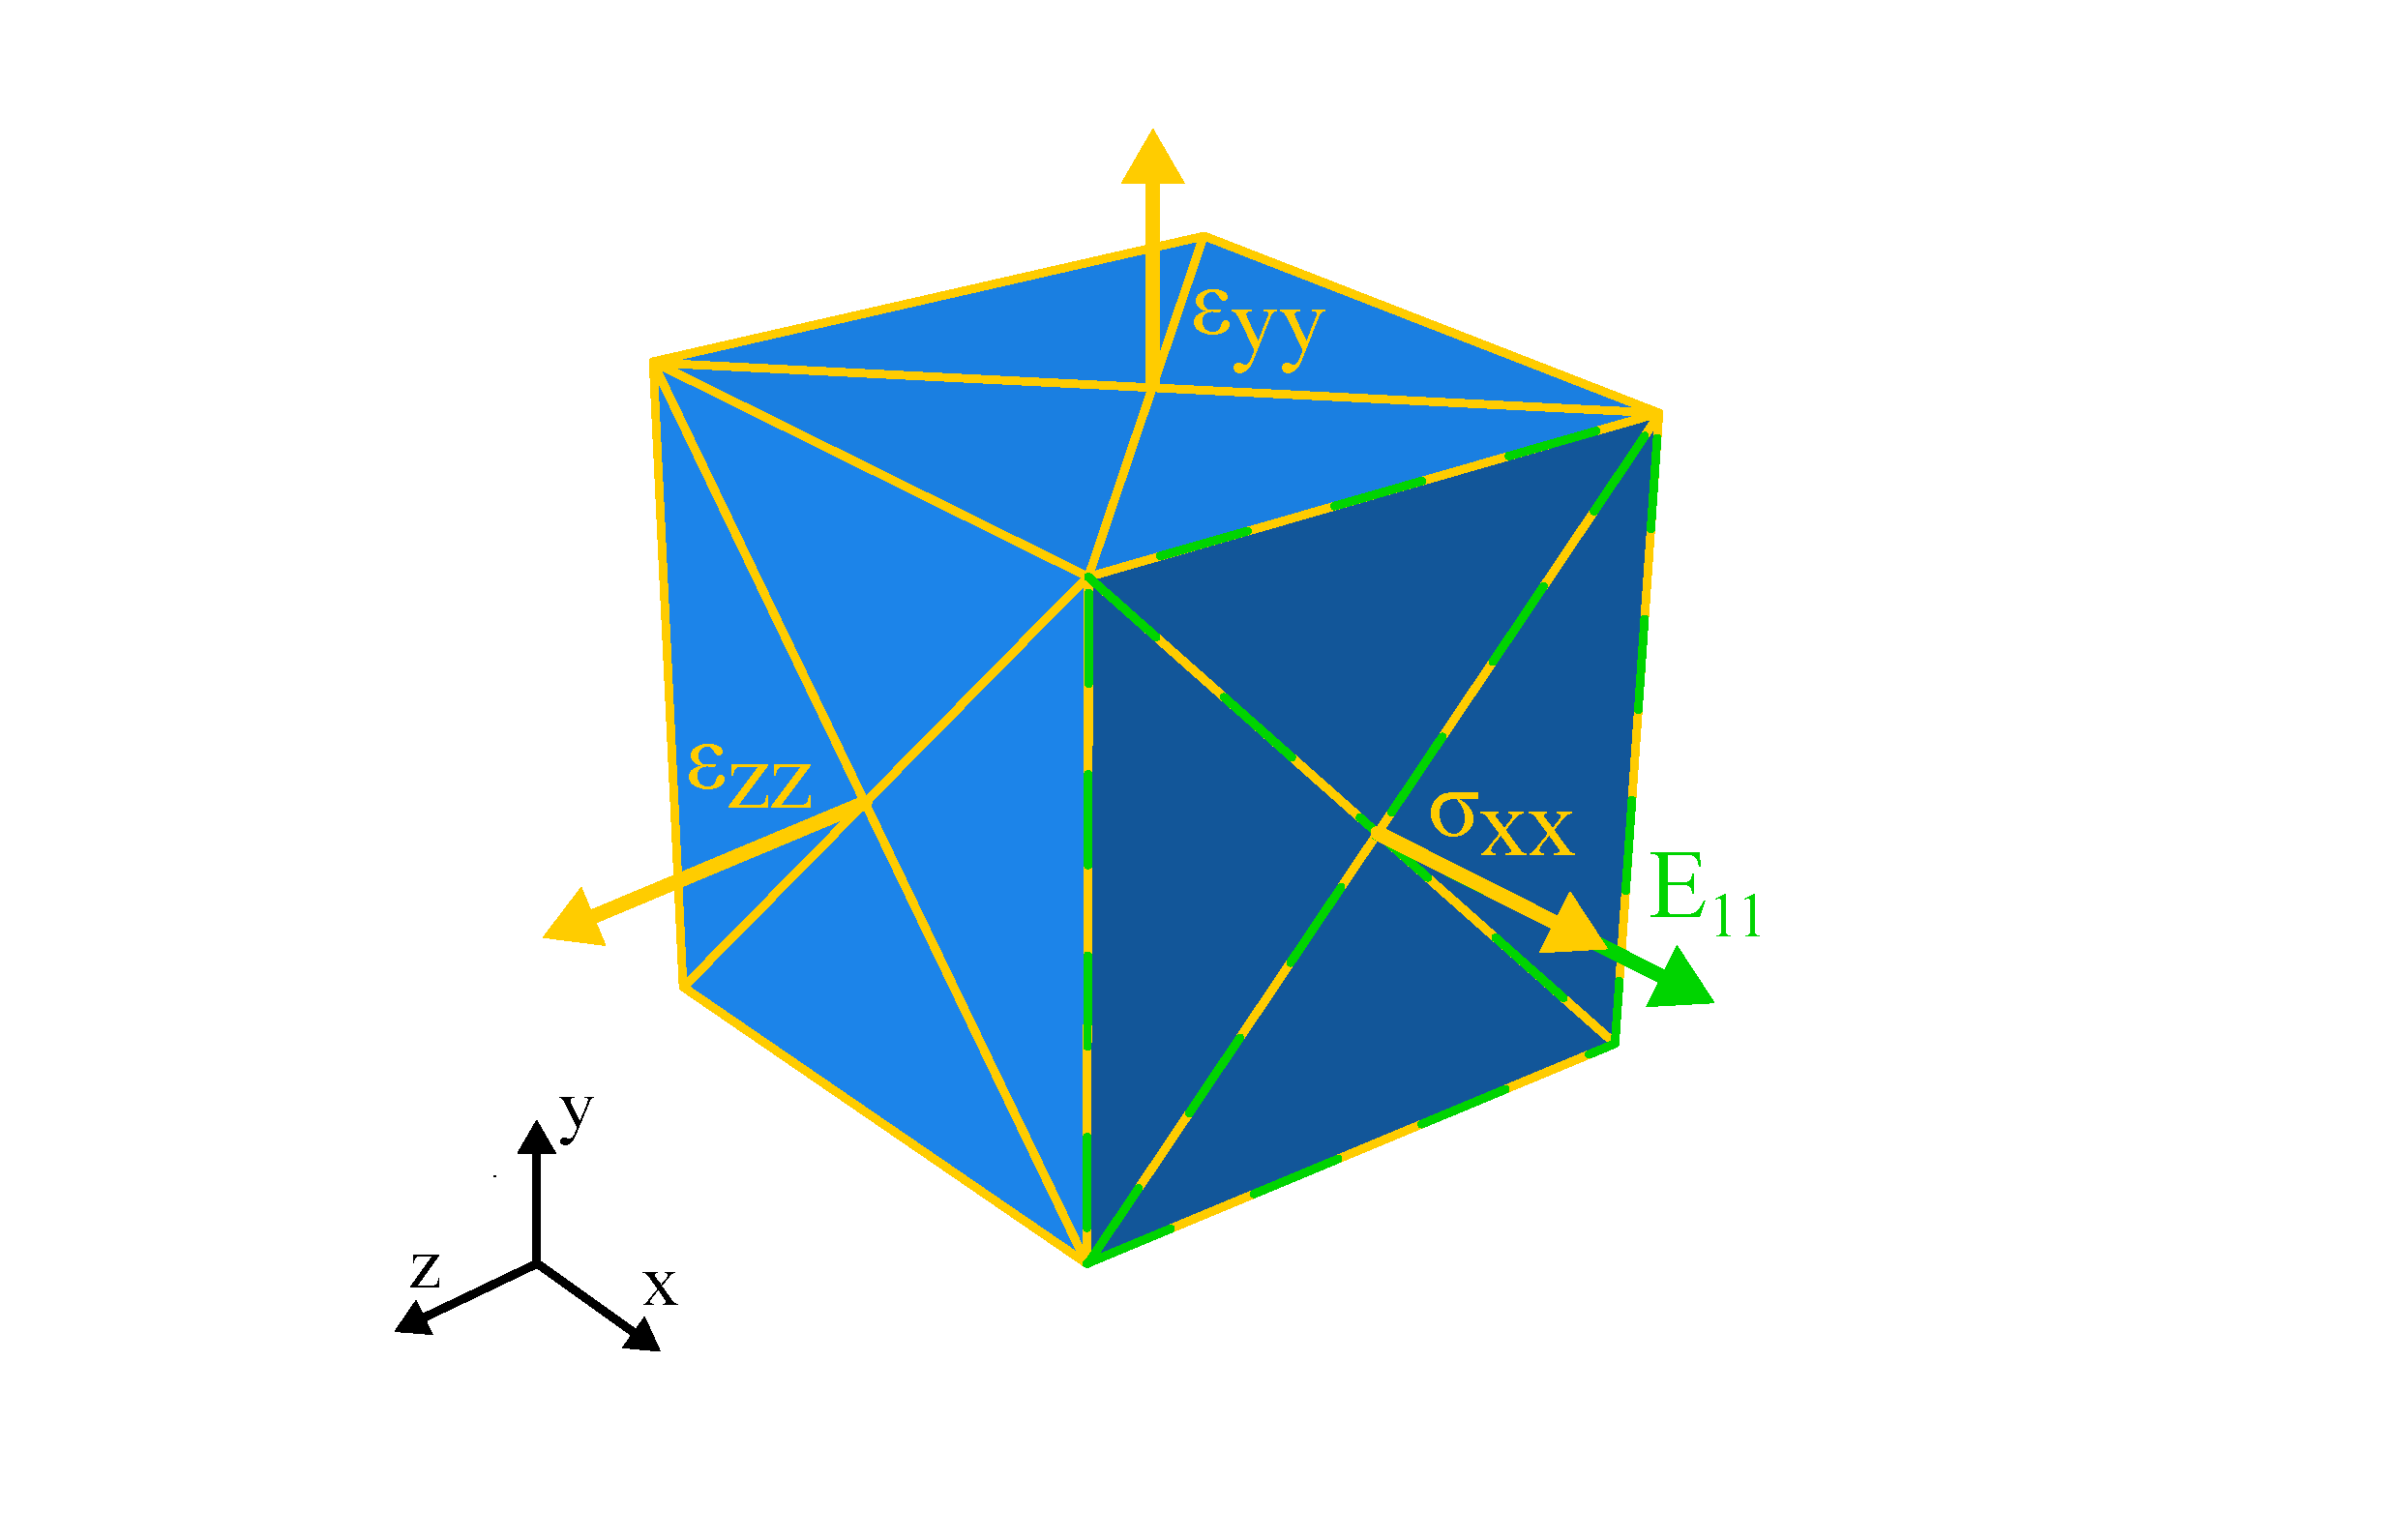
\includegraphics[width=0.7\textwidth]{cube_loading_plain_white_new.pdf}
    \caption{Illustration of exemplary load case E11 acting on the front surface in $xx$-direction (represented in green) with its exemplary evaluated stress and strain reactions $\sigma_{xx}, \varepsilon_{yy}$ and $\varepsilon_{zz}$ on the surfaces (represented in yellow)}
    \label{fig:evaluationMeasurements}
\end{figure}

\subsection{Load parameters and load reactions}\label{subsec:loadParameters}
For the optimisation process we use data from \acrshort{md} simulations as inputs.
This data are referenced as \emph{reference data} in the following. They contain stress and strain components for every time step from the \acrshort{md} simulation, in all normal and shear directions.
We split the reference data into \emph{load parameters} and \emph{\acrlong{rlr}}.
Load parameters refer to the quantitative values of the prescribed load case during the loading procedure.
Since we only process load cases identical to the ones in the \acrshort{md} simulations, we can transfer the load parameters directly in the \acrshort{fe} model.
A detailed description of the load application in \name{Abaqus} can be found in \autoref{sec: preprocessing}. \\
\indent The \acrlong{rlr} represent the material response during the \acrshort{md} simulation.
From these data we extract the stress and strain components according to the chosen \acrlong{er}, and neglect the remaining components, since they contain little information about the material behaviour.
As a result, we can register the \acrlong{rlr} for the corresponding load parameters to monitor the evolution of the material behaviour during the loading process.
To perform the inverse parameter identification, we need corresponding data from the \acrshort{fe} simulation.
In the way described in \autoref{sec: optimisationCode}, we can read out stress and strain components in all directions during the loading process.
Similar to the \acrlong{rlr} we extract the components corresponding to the \acrlong{er}.
These values are called \emph{\acrlong{olr}}. 
For an appropriate comparison, we must register the optimised and the \acrlong{rlr} at equivalent points in the loading period.
In \autoref{sec: preprocessing} we explain, how this is implemented in the script.

\paragraph{Application}
In \autoref{tab: testSeries}, the test series with their loading conditions are listed.
In the verification and validation studies, we apply linear strain up to a maximum value of 20 \%.
We analyse different mixing ratios in the validation studies, which demonstrate different mechanical behaviours.
As a preparation for studies with cyclic loading, we investigate a pure tensile strain following the first quarter sinus period over time with a maximum amplitude of 15 \% strain. With this loading trajectory, we study the optimisation behaviour for non-linear loading parameters.
We reuse this load parameters, and apply them as a shear strain in load case G12. Since in the previous tests always the load case E11 is used, we test the script performance for another load case.
To obtain more information about the material behaviour, we combine the load cases of E11 and G12 in one optimisation. 
As a last study we investigate one and a half period of a sinusoidal loading for a tensile load case in $xx$-direction. We use amplitudes of 1 \%, 5 \% and 8 \%. Important to notice is that the previously introduced load parameters proceed in a wide strain range. Assuming that the material starts to plastify quite fast, the majority of the loading steps are located in the plastic domain of the material. Conversely, the load parameters contain only little information about the elastic material behaviour. 
Through the use of load parameters with small amplitudes, we try to get a larger proportion of data points in the elastic domain.
In \autoref{sec: verification} the issue about this unequal distribution in the material domains becomes clear.    

\begin{table}[H]
    \centering
    \renewcommand{\arraystretch}{1.3}
    \caption{Overview of test series with corresponding loading conditions, materials and evaluated reactions}
    \label{tab: testSeries}
    \begin{tabular}{L{0.17\textwidth}C{0.08\textwidth}C{0.13\textwidth}C{0.15\textwidth}C{0.13\textwidth}C{0.17\textwidth}}
    \toprule
    \multirow{2}{0.17\textwidth}{\textbf{Test series}} & \multirow{2}{0.08\textwidth}{\centering \textbf{Load case}} & \multicolumn{2}{C{0.28\textwidth}}{\textbf{\ Load parameters}} &  \multicolumn{1}{C{0.13\textwidth}}{\multirow{2}{0.13\textwidth}{\centering \textbf{Mixing ratio}}} &\multirow{2}{0.17\textwidth}{\centering \textbf{Evaluated reaction}} \\ \cmidrule{3-4}
    & &\textbf{Trajectory} & \textbf{Amplitude} & & \\  \midrule
    Verification & E11 & Linear & 20\% & 6:3 & \(\sigma_{xx}, \varepsilon_{yy}, \varepsilon_{zz}\)\\\hline
    Validation I & E11 & Linear & 20\% & 4:3 & \(\sigma_{xx}, \varepsilon_{yy}, \varepsilon_{zz}\)\\ \hline
    Validation II& E11 & Linear & 20\% & 6:3 & \(\sigma_{xx}, \varepsilon_{yy}, \varepsilon_{zz}\)\\ \hline
    Validation III& E11 & Linear & 20\% & 8:3 & \(\sigma_{xx}, \varepsilon_{yy}, \varepsilon_{zz}\)\\ \toprule
    \multirow{2}{0.15\textwidth}{Pure tensile strain} & E11 & Sinus (\(\frac{1}{2} \pi\)) & 15\% & 6:3 & \(\sigma_{xx}, \varepsilon_{yy}, \varepsilon_{zz}\)\\ 
            &   &           &   && \\ \hline
    Simple shear strain  & G12 & Sinus (\(\frac{1}{2}\pi\)) & 15\% & 6:3 & \(\sigma_{xy}\)\\ \hline
    \multirow{2}{0.15\textwidth}{Tensile \& Shear strain} & E11 & Sinus (\(\frac{1}{2}\pi\)) & 15\% & 6:3 & \(\sigma_{xx}, \varepsilon_{yy}, \varepsilon_{zz}, \sigma_{xy}\)\\ 
                            & G12 &       &      &     \\ \hline
    \multirow{2}{0.15\textwidth}{Cyclic tensile strain} & E11 & Sinus (\(3\pi\)) & 1\%  & 6:3 & \(\sigma_{xx}, \varepsilon_{yy}, \varepsilon_{zz}\)\\ 
                &     &       & 5\%  &  & \(\sigma_{xx}, \varepsilon_{yy}, \varepsilon_{zz}\)\\ 
                &     &       & 8\%  & & \(\sigma_{xx}, \varepsilon_{yy}, \varepsilon_{zz}\)\\ \bottomrule
    \end{tabular}
    
\end{table}



\section{Error Calculation}\label{sec: errorCalculation}
For a representative value including all necessary data, we select the \acrshort{rmse}, which is explained in \autoref{subsec: RMSE}.
We insert the \acrlong{rlr} and the \acrlong{olr} as data sets in \autoref{eq: multiRMSE}.
The extraction of the load reactions from the \acrshort{fe} simulation is described in \autoref{sec: optimisationCode}.
The access to \acrlong{rlr} is explained in \autoref{subsec:loadParameters}.
We compute the deviations of the \acrlong{olr} at each load step. \autoref{fig: erroPlot} displays this procedure for an exemplary set of \acrlong{rlr} and \acrlong{olr}. Here $\sigma_{xx}$ is the selected \acrlong{er}.
For every load step LS their corresponding \acrfull{rlr} $\sigma_{\scriptscriptstyle\text{LS}}^{\scriptscriptstyle\text{RLR}}$ and \acrfull{olr} $\sigma_{\scriptscriptstyle\text{LS}}^{\scriptscriptstyle\text{OLR}}$ are logged. The blue arrow highlights their deviation $\Delta\sigma_{\scriptscriptstyle\text{LS}}$ for one exemplary load step, according to \autoref{eq: EMDifference}. 
As described in \autoref{subsec:loadParameters}, the distribution of the data points is unfavourable for the determination of the elastic parameters. 
To support the script in finding the elastic parameters, we applied a weight of 100 at the data point in the elastic domain, i.e. below 1 \% strain. This is done via an array $\boldsymbol{w}$ which entries are one except the first entry $w_{\scriptscriptstyle\text{1}}$. Formally, the applied weights have the inverse unit of the evaluated load reaction, i.e. for stress load reactions, $[w_{\text{LS}}] = \text{MPa}^{-1}$ would be the correct unit for the related weights.
According to \autoref{eq: mse}, we calculate the mean value of the weighted arrays.
The resulting value is called \emph{\acrfull{mse}} for one \acrlong{er}. We compute $\text{MSE}_{\sigma}$ or $\text{MSE}_{\varepsilon}$ for every selected \acrlong{er}. 

\begin{figure}[H]
    \centering
    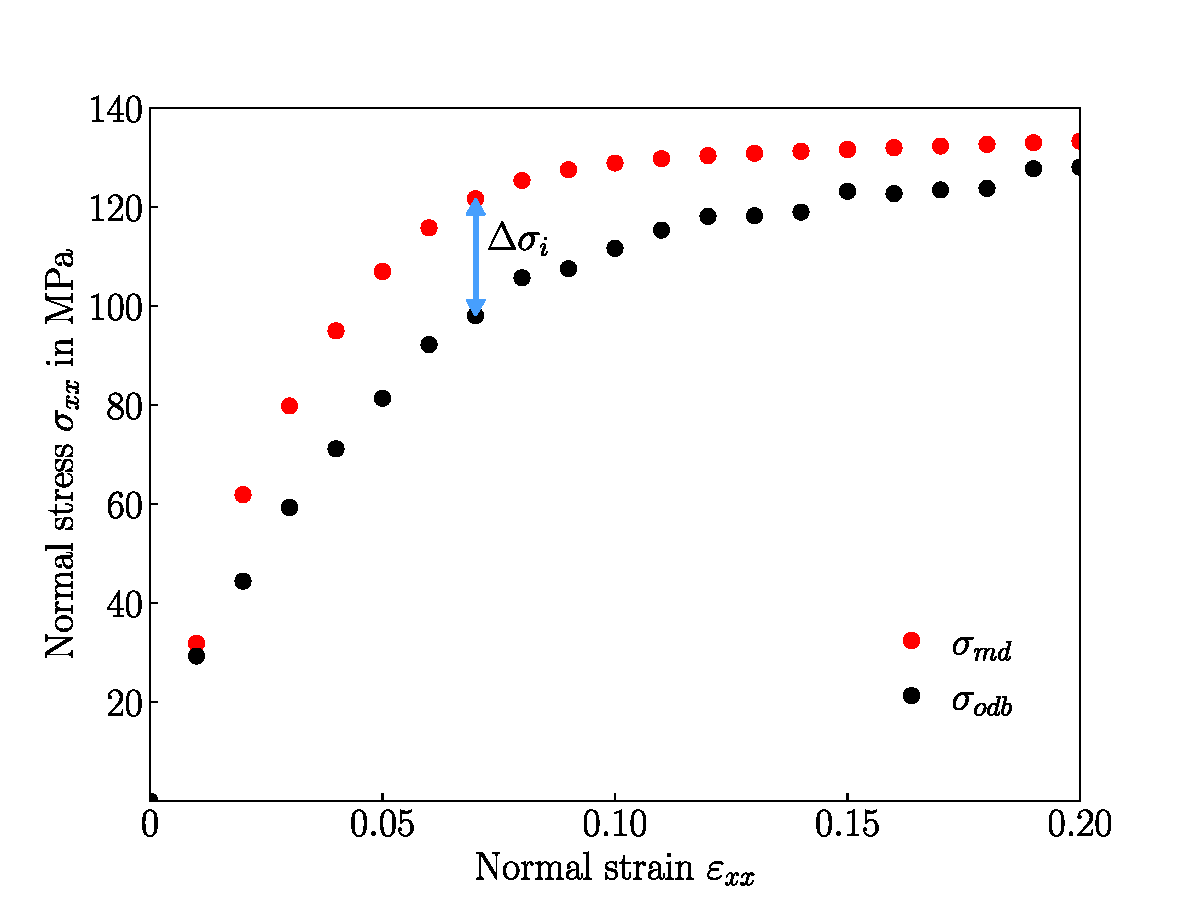
\includegraphics[width = 0.65\textwidth]{error_plot.pdf}
    \caption{Exemplary \acrlong{rlr} $\sigma^{\scriptscriptstyle\text{RLR}}$ and \acrlong{olr} $\sigma^{\scriptscriptstyle\text{OLR}}$ with visualization of error calculation}
    \label{fig: erroPlot}
\end{figure}
XX FIGURE ANPASSEN

\begin{gather}
    \label{eq: EMDifference}
    \Delta\sigma_{\scriptscriptstyle\text{LS}} = \sigma_{\scriptscriptstyle\text{LS}}^{\scriptscriptstyle\text{RLR}} - \sigma_{\scriptscriptstyle\text{LS}}^{\scriptscriptstyle\text{OLR}} \hspace{2cm}
    \Delta\varepsilon_{\scriptscriptstyle\text{LS}} = \varepsilon_{\scriptscriptstyle\text{LS}}^{\scriptscriptstyle\text{RLR}} - \varepsilon_{\scriptscriptstyle\text{LS}}^{\scriptscriptstyle\text{OLR}}\\
    \label{eq: mse}
    \text{MSE}_{\sigma} = \frac{\displaystyle\sum_{\text{LS}} w_{\scriptscriptstyle\text{LS}} (\Delta\sigma_{\scriptscriptstyle\text{LS}}^2)}{\displaystyle\sum_{\text{LS}}w_{\scriptscriptstyle\text{LS}} } \hspace{2cm}
    \text{MSE}_{\varepsilon} = \frac{\displaystyle\sum_{\text{LS}} w_{\scriptscriptstyle\text{LS}} (\Delta\varepsilon_{\scriptscriptstyle\text{LS}})^2}{\displaystyle\sum_{\text{LS}}w_{\scriptscriptstyle\text{LS}}}
\end{gather}

For the tensile load case for example, we must perform this for the \acrlong{er} $\sigma_{xx}, \varepsilon_{yy} \text{ and } \varepsilon_{zz}$. 
In order to construct a single error value of these \acrshort{mse}s, we must ensure a common scale. Otherwise, their influence on the overall error may vary significantly.
In general, the \acrshort{mse}s of \acrlong{eer} are much smaller than the ones from \acrlong{esr}, such that loading dependent weights $w_{\sigma}$ and $w_{\varepsilon}$ are introduced. 
The exact weights depend on the load case and the used load parameter set.
From the weighted \acrshort{mse} we construct the \acrshort{rmse} as shown in \autoref{eq: rmse}. 
Since the code is able to process multiple load cases in one optimisation process, we can calculate the \acrshort{rmse} for every load case and apply associated weights $w_{\scriptscriptstyle\text{LC}}$. Additionally, multiple load parameters sets (LP) can be processed, which leads to \acrshort{rmse} values for every load parameter set with the weight $w_{\scriptscriptstyle\text{LP}}$. 
As stated in \autoref{eq: error}, we assemble the individual \acrshort{rmse}s in a double sum over the load cases and the load parameter sets. This \benennung{Error} is the value we return the numerical optimisation algorithm. In the following sections we have a closer look at the implementation of this minimisation process. 

\begin{gather}
    \label{eq: rmse}
        \text{RMSE} = \sqrt{\frac{\displaystyle\sum_{\text{ESR}} w_{\sigma} \cdot \text{MSE}_{\sigma} + \displaystyle\sum_{\text{EER}} w_{\varepsilon} \cdot \text{MSE}_{\varepsilon}}{N_\text{ESR} + N_\text{EER}}} \\
        \label{eq: error}
    \text{Error} = \sum_{\text{LP}} \sum_{\text{LC}} w_{\scriptscriptstyle\text{LP}} w_{\scriptscriptstyle\text{LC}} \cdot \text{RMSE}_{\scriptscriptstyle \text{LC}, \text{LP}} \\
        N_\text{ESR}: \text{Number of \acrlong{esr}} \nonumber\\
    N_\text{EER}: \text{Number of \acrlong{eer}} \nonumber
\end{gather}


\section{Preprocessing} \label{sec: preprocessing}
Before starting with the optimisation process, we need preprocessing steps to create a working \name{Abaqus} model with the required properties. The user-defined properties are transferred in an input-file. \autoref{tab: inputParameterTable} lists an extract of this file, containing only parameters relevant for the optimisation process.
\begin{table}[H]
    \centering
    \caption{Input parameters for optimisation process}
    \label{tab: inputParameterTable}
    \renewcommand{\arraystretch}{1.1}
    \begin{tabular}{L{0.2\textwidth}C{0.2\textwidth}C{0.15\textwidth}C{0.1\textwidth}C{0.1\textwidth}}
    \toprule
    \textbf{Input parameter} & \textbf{Directions} & \textbf{Category} & \textbf{Data format} & \textbf{Unit} \\ \midrule
    Young's modulus & – & value    & array  & MPa \\ 
                & – & minimum  & scalar & MPa \\ 
                & – & maximum  & scalar & MPa \\ \hline
    Poisson's ratio  & – & value    & array  & –   \\ 
                & – & minimum  & scalar & –   \\ 
                & – & maximum  & scalar & –   \\ \hline
    Yield stress  & – & value    & array  & MPa \\ 
                & – & minimum  & scalar & MPa \\ 
                & – & maximum  & scalar & MPa \\ \hline
    \multirow{2}{0.2\textwidth}{Alpha, beta, gamma} & – & value    & array  & –   \\ 
                    & – & minimum  & scalar & –   \\ 
                    & – & maximum  & scalar & –   \\ \hline
    Load parameters & – & filename & string & –   \\ 
                    & – & weight   & scalar & –   \\ \hline
    Load case & \multirow{2}{0.2\textwidth}{E11, E22, E33, G12, G23, G13} & active & boolean    & – \\ 
            &                               & weight & scalar & – \\ \hline
    Stress evaluation & \multirow{2}{0.15\textwidth}{$xx$, $yy$, $zz$, $xy$, $yz$, $xz$} & active & boolean   & – \\ 
                    &                        & weight & scalar & – \\ \hline
    Strain evaluation & \multirow{2}{0.15\textwidth}{$xx$, $yy$, $zz$, $xy$, $yz$, $xz$} & active & boolean  & – \\ 
                    &                        & weight & scalar & – \\ \hline
    Load weighting & \multirow{4}{0.2\textwidth}{normal stress, normal strain, shear stress, shear strain} & weight & scalar & – \\ 
    &&&& \\
    &&&& \\
    &&&& \\\bottomrule
    \end{tabular}
    
\end{table}

The input file contains more parameters for different namings, which are neglected here. In attaachment XX the whole input file is included. 
The user has multiple options to configure the optimisation process. It is possible to test multiple initial value combinations for the material parameters calling the script once. In \autoref{tab: inputParameterTable} this is visible in the column \benennung{Data format} for the material parameters.
Here, the user can pass an array with multiple initial value for every material parameter.
This function is important to validate the optimisation results with varying input values. \\
\indent In \autoref{fig: flowchart} the complete structure of the code is depicted. The white boxes show the individual phases referred to in the text in italics. The coloured boxes represent the performed loops. 
The upper part belongs to the preprocessing, which starts with the phase \benennung{Read input file}. \\
\indent In this phase all entries from the input-file are extracted. 
To process the arrays with the initial material parameters, the script loops over all arrays at a time to extract one initial value for each parameter.
The entries with the same index result in one initial value combination which is visualised in \autoref{tab:material_combinations}.
As a consequence, all arrays need to be of same length. For every initial value combinations the script creates a new \acrfull{mdb} in \name{Abaqus}, and a new folder structure to set the working directory and store the results.

\begin{table}[h!]
    \centering
    \caption{Loop conditions in preprocessing}
    \label{tab:loop_conditions}
    \begin{subtable}[t]{0.45\textwidth}
        \centering
        \renewcommand{\arraystretch}{1.1}
        \caption{Exemplary arrangement of initial value combination of material parameters for five combinations}
        \label{tab:material_combinations}
        \begin{tabular}{L{0.31\textwidth}|C{0.08\textwidth}C{0.08\textwidth}C{0.08\textwidth}C{0.08\textwidth}C{0.08\textwidth}}
            \toprule
            \multirow{2}{0.31\textwidth}{\textbf{Material Parameter}} & \multicolumn{5}{c}{\textbf{Combination}} \\
            \cmidrule(lr){2-6}
             & \textbf{1} & \textbf{2} & \textbf{3} & \textbf{4} & \textbf{5} \\ \midrule
            $E$ & $E_1$ & $E_2$ & $E_3$ & $E_4$ & $E_5$ \\ \hline
            $\nu$ & $\nu_1$ & $\nu_2$ & $\nu_3$ & $\nu_4$ & $\nu_5$ \\\hline
            $\sigma_0$ & $\sigma_{0_1}$ & $\sigma_{0_2}$ & $\sigma_{0_3}$ & $\sigma_{0_4}$ & $\sigma_{0_5}$ \\\hline
            $\alpha$ & $\alpha_1$ & $\alpha_2$ & $\alpha_3$ & $\alpha_4$ & $\alpha_5$ \\\hline
            $\beta$ & $\beta_1$ & $\beta_2$ & $\beta_3$ & $\beta_4$ & $\beta_5$ \\\hline
            $\gamma$ & $\gamma_1$ & $\gamma_2$ & $\gamma_3$ & $\gamma_4$ & $\gamma_5$ \\ 
            \bottomrule
        \end{tabular}
    \end{subtable}  
    \hfill
    \begin{subtable}[t]{0.45\textwidth}
        \centering
        \renewcommand{\arraystretch}{1.17}
        \caption{Exemplary model creation for two load cases E11 and G12 in combination with three load parameter sets}
        \label{tab:model_creation}
        \begin{tabular}{L{0.25\textwidth}|C{0.2\textwidth}C{0.35\textwidth}}
            \toprule
            {\textbf{Model}} & \textbf{Load case} &  \textbf{Load parameters} \\ \midrule
            Model 0 & E11 & Data set 1 \\ \hline
            Model 1 & E11 & Data set 2 \\\hline
            Model 2 & E11 & Data set 3 \\\hline
            Model 3 & G12 & Data set 1 \\\hline
            Model 4 & G12 & Data set 2 \\\hline
            Model 5 & G12 & Data set 3 \\
            \bottomrule
        \end{tabular}
    \end{subtable}    
\end{table}

We start the first loop with the phase \benennung{Create model}. As discussed in \autoref{sec: FEMBasics}, we model a cube with size 1x1x1. We mesh the cube with 6x6x6 elements. Because of the regular geometry, discretising with hexagonal structured elements is feasible.
The number of elements is a compromise between a coarse mesh for fast computation and a minimum number to avoid convergence errors.
Although we use a hyperelastic material in our optimisation process, we first apply an elastic material.
We assign isotropic behaviour and attribute $E$ and $\nu$ their initial values. \\
\indent The elastic material is necessary because of the usage of EasyPBC in the phase \benennung{Create job}.
We start EasyPBC, which creates a job with the load case prescribe in the input.
As discussed in \autoref{subsec: EasPBC}, we use EasyPBC for the automatic construction of \acrshort{pbc}. Aside from that, we adopt the generated load application corresponding to the load case. \\
\indent However, the settings from EasyPBC contain some default values, we adjust in the phase \benennung{Modify properties}. EasyPBC applies for every load case a uniform displacement with a constant default value.
We need to adopt this value, since we want to apply the loading parameters from the \acrshort{md} simulations, which are not constant.
In \name{Abaqus} we can solve this issue by creating an \emph{amplitude} to apply the load gradually (see \autoref{fig:amplitudemenu}).
Therefore, we enter the load parameters as an amplitude at certain time steps.
For the time steps we use sequential numbering. We use these time steps later to adapt the evaluation points of the \acrlong{olr}.
The value in the boundary condition editor is then set to one because this only defines the factor by which the amplitude is multiplied (see \autoref{fig:bcmenu}).
As a result, the load is applied step-wise with step sizes defined through the amplitude values, i.e. the load parameters. 
In the \name{Abaqus} environment, these steps are referenced as \emph{load steps}.\\
\indent We use the time steps, created in the amplitude menu as request points for the \acrlong{olr}.
Thus, at every time step the \acrlong{olr} caused by the corresponding load step are written. 
Through the transfer of the load steps from the reference data, the reference and the optimised load reactions are written at equivalent evaluation points in the loading process.\\
\indent Afterwards, we modify the increment settings.
EasyPBC automatically creates increments with fixed size and without non-linear geometry effects. 
In order to avoid convergence errors, we use automatic incrementation.
Especially in the first load steps, we observe large deformations.
If we try to resolve such large deformations in one incrementation step, \name{Abaqus} runs into convergence errors.
With automatic incrementation, \name{Abaqus} can dynamically adapt the number of increments per load step depending on the current deformation. The non-linear geometry effects must be considered for the same reason. \\
\indent In the last step of preprocessing we \emph{store} the model in a dictionary. We use this dictionary later to call the models for the optimisation.
We perform the preprocessing for all prescribed load cases which is highlighted in the green loop in \autoref{fig: flowchart}. Furthermore, the purple area in \autoref{fig: flowchart} visualises the loop over the load parameters. This leads to individual models for every load case and every load parameter set, which is exemplary listed for two load cases and three load parameter sets in \autoref{tab:model_creation}.

\begin{figure}[H]
    \centering
    % --- Subfigure (a)
    \begin{subfigure}[t]{0.35\textwidth}
        \centering
        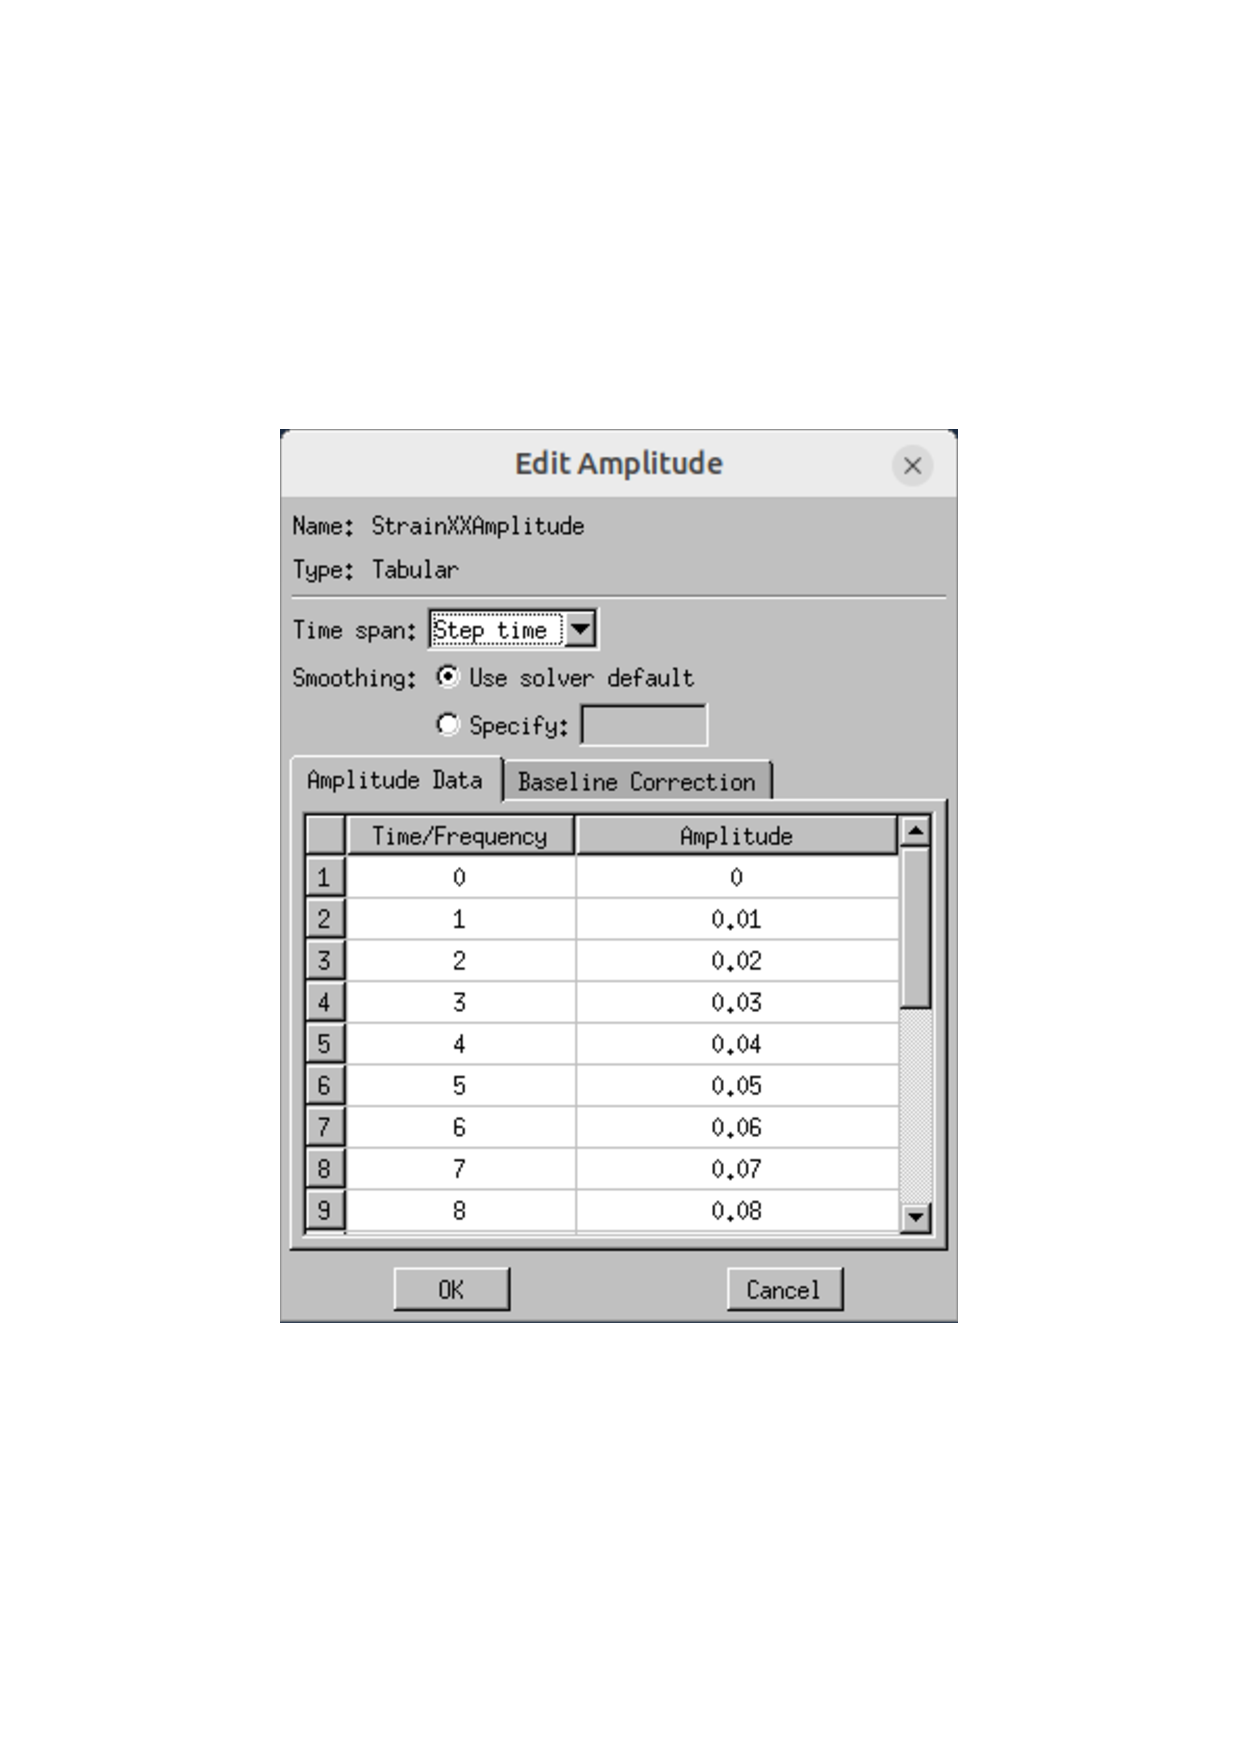
\includegraphics[width=\linewidth]{Amplitude.pdf}
        \vfill{}
        \caption{ Definition of load amplitude in \name{Abaqus}} % eigene (a)-Caption
        \label{fig:amplitudemenu}
    \end{subfigure}
    \hspace{0.08\textwidth}
    % --- Subfigure (b)
    \begin{subfigure}[t]{0.35\textwidth}
        \centering
        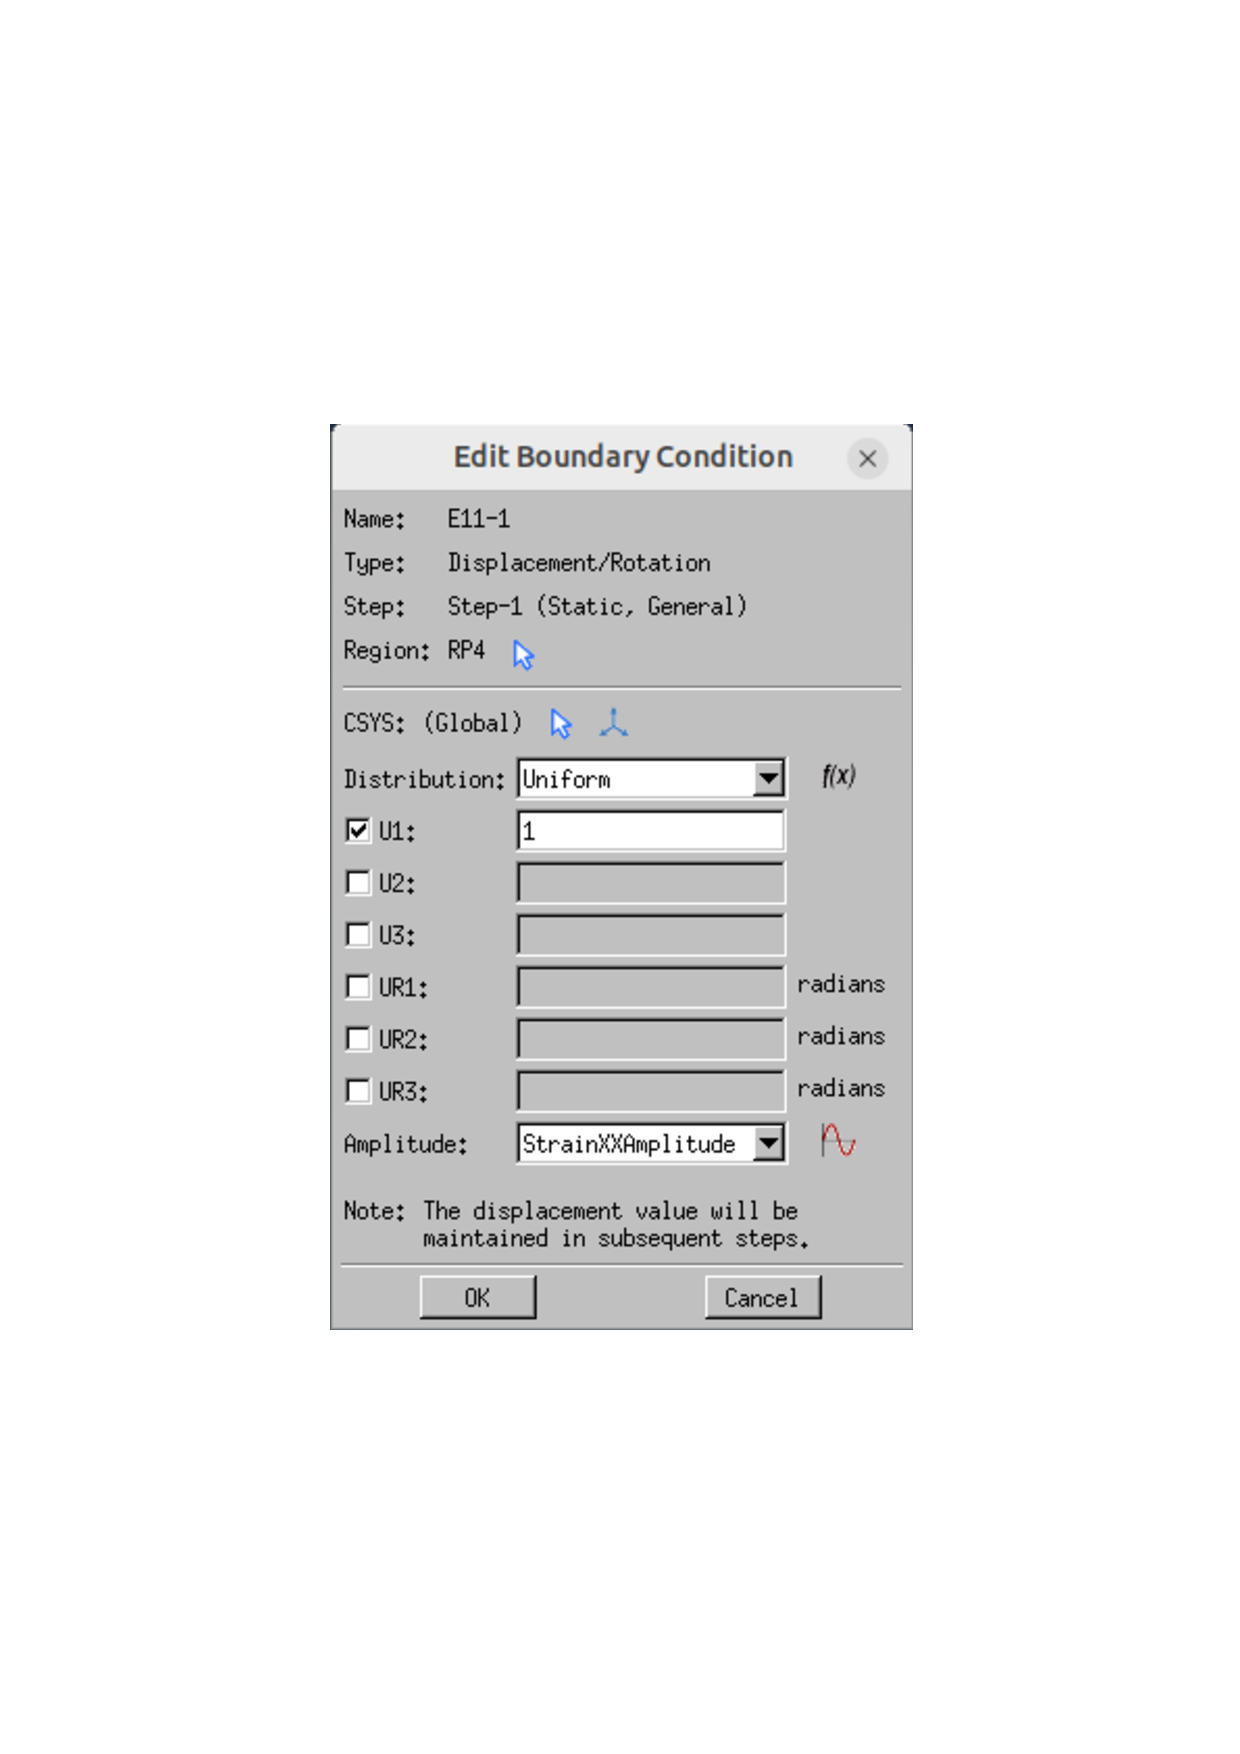
\includegraphics[width=\linewidth]{BC.pdf}
        \caption{Boundary condition menu in \name{Abaqus}}
        \label{fig:bcmenu}
    \end{subfigure}

    \caption{Loop conditions in preprocessing}
    \label{fig:abaqus_settings}
\end{figure}

\section{Optimisation process} \label{sec: optimisationCode}

\begin{figure}[H]
    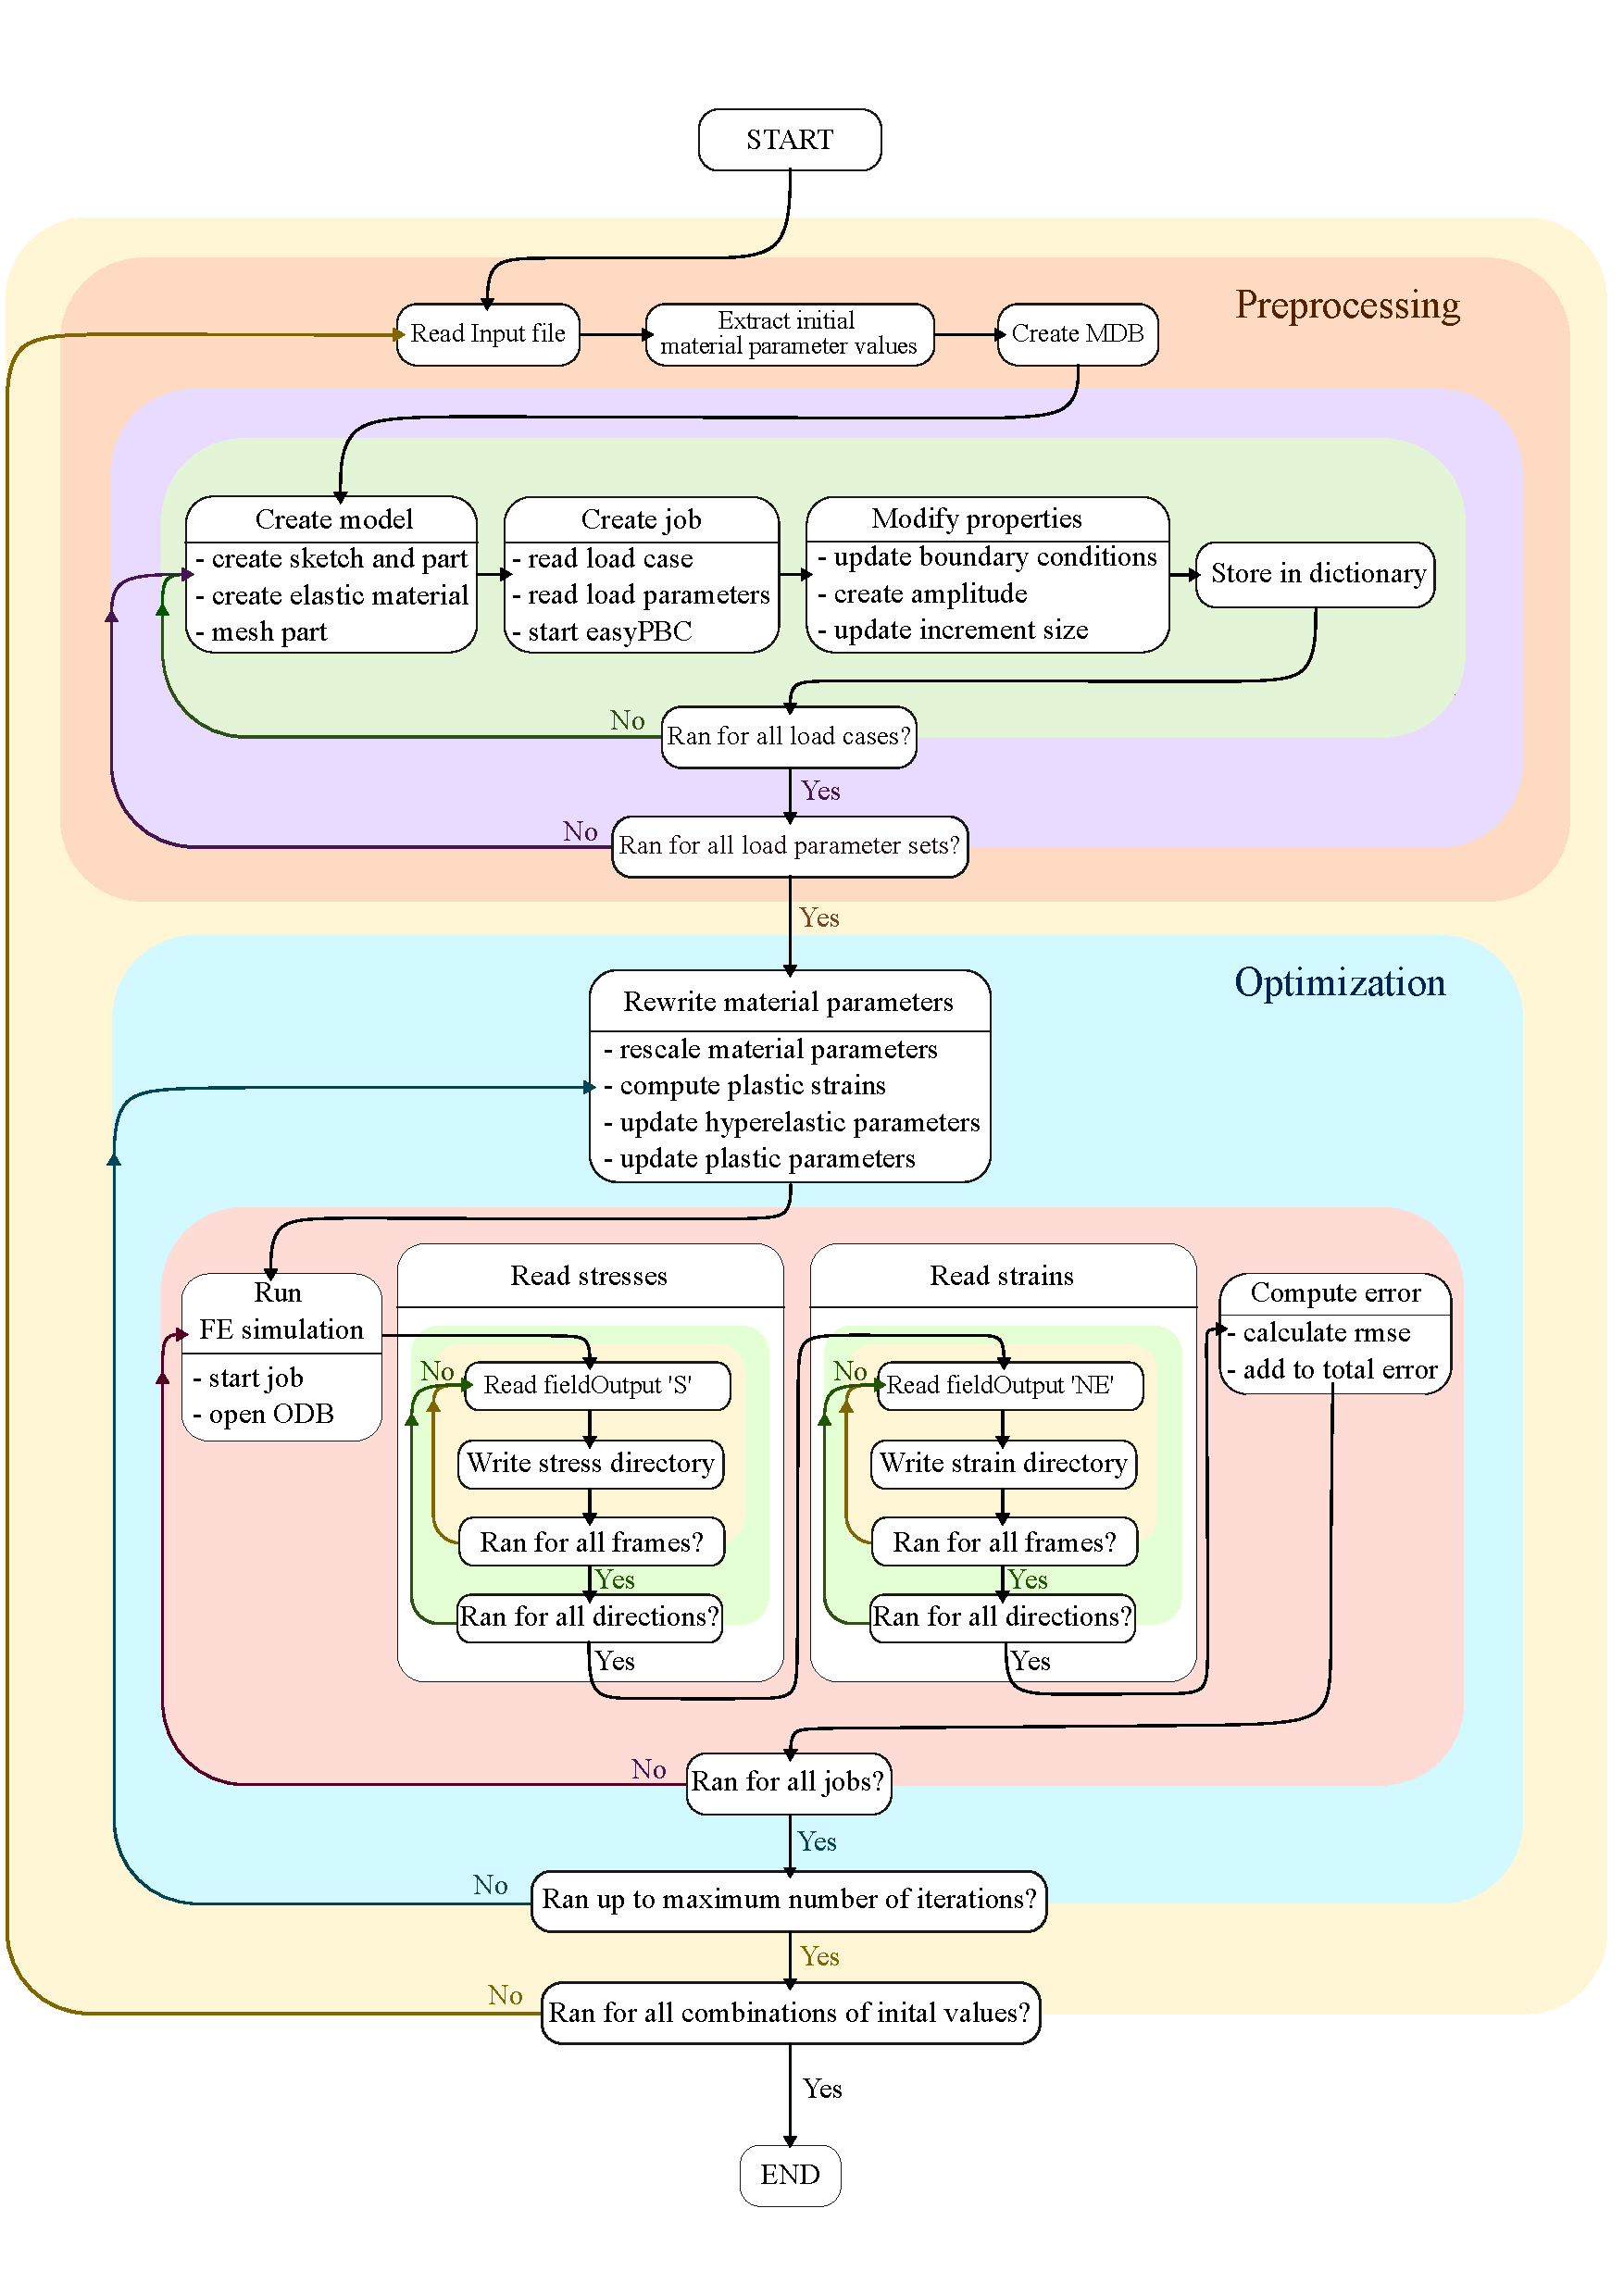
\includegraphics[width = 1.0\textwidth]{complete_flowchart_new.pdf}
    \caption{Flowchart code}
    \label{fig: flowchart}
\end{figure}

\begin{table}[h!]
\centering
\renewcommand{\arraystretch}{1.2}
\caption{List of general input parameters for the scipy.minimize-function with the contents passed in the function-call}
\label{tab: minimizeFunctionInput}
\begin{tabular}{L{0.15\textwidth}|L{0.2\textwidth}C{0.12\textwidth}L{0.4\textwidth}}
\toprule
\textbf{Parameter} & \textbf{Content} & \textbf{Data format} & \textbf{Explanation} \\
\midrule
Objective function & Optimisation function & -- & Function whose scalar value should be minimized \\ \hline

Initial guess & Material parameters & array & Scaled initial values for the optimisation parameters \\\hline

\multirow{2}{0.15\textwidth}{Additional arguments}
 & Cube parameters & object & Model information from input file \\
 & Load parameters & dictionary & Load parameters from MD-simulations \\
 & Work directory & string & Path to store results \\
 & Evaluation counter & scalar & Counter for the performed function evaluations \\ \hline

method & Nelder-Mead & -- & Numerical algorithm \\\hline

bounds & Limits for material parameter & array & Upper and lower boundary values for every optimisation parameter \\\hline

maxiter & Number of iterations & scalar & Maximum number of iterations  as termination criterion\\
\bottomrule
\end{tabular}
\end{table}

In the following section, we describe the optimisation process. We start the process by calling the \verb|scipy.minimize|-function. We pass this function various parameters, listed in \autoref{tab: minimizeFunctionInput}. The \verb|scipy.minimize|-function calls our self-written optimisation function, where the evaluation takes place. The \emph{initial guess} stores an array with start values for all parameters that should be optimised. Additionally, we pass information about the models that we created in the preprocessing and the load parameters. We use all models created in the preprocessing for one optimisation call. \\
\indent We start the process with the phase \benennung{Rewrite material parameters} for all models.
Since they all describe the same material, we write the same values for every model.
For a better performance of the Nelder-Mead algorithm, the optimisation parameters are scaled in the bounds from zero to one.
To rewrite the values in the models, we have to rescale them first.
Then, we can use the rescaled parameters to compute the values for the hardening-function with the formula for VOCE-hardening (\autoref{eq: voce}).
We remove the elastic material and substitute it with a hyperelastic material which is suitable for high non-linear deformations.
To achieve this, we convert the Young's modulus and the Poisson's ratio into the hyperelastic parameters $C_{10}$ and $D_1$ via the relations
\begin{gather}\label{eq: elasticParams}
    C_{10} = \frac{E}{4(1+ \nu)} \hspace{1.5cm}
    D_1 = \frac{6(1-2\nu)}{E}.
\end{gather}

Now we can update the material parameters in all models. In the next steps, we handle the models successively.
We start the job of the first model to perform the \name{Abaqus} analysis and open the resulting \emph{\acrfull{odb}} in the \benennung{Run FE-simulation} phase. In the \acrshort{odb} all simulation results are stored.\\
\indent With the phase \benennung{Read stresses} the evaluation begins. First, we read the \emph{FieldOutput} variable 'S' and write the data in a directory. In the FieldOutput, \name{Abaqus} stores the values of various quantities, e.g. stresses, strains and energy components, during the simulation.
The variable 'S' contains the stress components in all directions, i.e. the stress components of the optimised load reactions.
We read out every \emph{frame} from the \acrshort{odb}, since one frame corresponds with one load step.
Additionally, we loop over all directions ($xx$, $yy$, $zz$, $xy$, $yz$, $xz$). \\
\indent We employ the same for the strain values in the phase \benennung{Read strains}.
Here it is important to read out the correct strain variable 'NE' (nominal strain).
For hyperelastic materials, \name{Abaqus} uses the logarithmic strain ('LE') as standard value. Because of its logarithmic scaling, we cannot compare them to the reference data. We store all values for all frames and directions in a dictionary, similar to the stress values.
Consequently, all \acrlong{olr} are stored, and the step \benennung{Compute error} can be executed. \\
\indent In this step, the error is computed as described in \autoref{sec: errorCalculation}.
For a better structure of the code this part is captured in a separate function.
We call this function, and pass the \acrlong{olr} and load parameters.
The function compute the \acrshort{rmse} according to \autoref{eq: rmse} and returns it.
Multiplied with its corresponding weights for the load case and the load parameters, we add this value to the total error according to \autoref{eq: multiRMSE}.
Now we restart the \emph{job loop} in \autoref{fig: flowchart} by starting the FE-simulation for the next job.
Once all the jobs are processed, and we computed the total error value, we return it to our minimisation function.
The internal Nelder-Mead algorithm reduces the error and returns the corresponding material parameters.
This completes one optimisation iteration. In \autoref{fig: flowchart}, the \emph{iteration loop} is visualised with the blue box.
This process will run until the defined number of maximum iterations is exceeded, or convergence is reached. When the changes in the total error are very small, the internal convergence criterion is reached and the algorithm stops.


\section{Data storage} \label{sec: dataStorage}

To evaluate the optimisation process at the end, parameter values need to be recorded during the preprocessing and the optimisation process.
This ensures that the values of all iterations are saved, since the variable values are rewritten in every new iteration.
In the preprocessing, we extract the current initial value combination from the input file. \\
\indent All files created from \name{Abaqus} like the CAE, \acrshort{odb} and the job-files are stored in a subfolder.
In the optimisation part, multiple functions are called after the phase \benennung{Compute error} to store the current variable values. The material parameters for every iteration are stored. In addition, we store multiple interim results during the error calculation. For every job the weighted \acrshort{mse}s are stored for every iteration, so that the impact and evolution of every evaluated reactions can be understood. To track the impact of the applied weights, all \acrshort{rmse} values are stored individually and weighted. In addition, we store the total error, which is the sum of all weighted \acrshort{rmse}s of one iteration. Finally, we have one file each for the material parameters, \acrshort{mse}s, \acrshort{rmse}s, and the total errors. All these files are handled in the same way. After the computation of the total error, the variable values of the current iteration are stored. The stress and strains are stored in separate files for each iteration. We create for each job a subfolder, where its stress and strain values are stored. For one iteration, a file is created which contains the stress and strain dictionaries from the steps \benennung{Read stress} and \benennung{Read strain}. This leads to as many files as iterations were performed for every job. At the end of the optimisation process, we store the final message returned from the Scipy.minimize function. \name{Python} automatically sends a message where the cause of termination is stated. This message becomes important if the algorithm stops before the maximum number of iterations is reached. Then we can reproduce whether this happens because the convergence limit is reached or a numerical error occurred. The described procedure to store the data is done for every initial value combination separately.

\begin{table}[H]
    \centering
    \renewcommand{\arraystretch}{1.2}
    \caption{Overview of the performed tests with corresponding input parameters}
    \label{tab:storageData}
    \begin{tabular}{L{0.3\textwidth}|C{0.1\textwidth}L{0.5\textwidth}}
    \toprule
   \textbf{Stored parameters} & \textbf{Data format} & \textbf{Explanation}\\ \midrule
   Input parameters & JSON & Copy of the input file with current initial value combination\\ \hline
   Material parameters & CSV & Table with all material parameters for each evaluation\\\hline
   weighted \acrshort{mse} & CSV & File per job with weighted \acrshort{mse} per evaluation \\\hline
   \acrshort{rmse} & CSV & File with \acrshort{rmse} per job, each stored alone, with weight for load case, and weight for load parameters \\\hline
   Total error & CSV & Total error after each evaluation \\\hline
   Optimised load reactions & CSV & File per job with all optimised load reactions in one evaluation \\\hline
   Scipy.minimize message & TXT & Final message about the termination status of the scipy-function\\
    \bottomrule
    \end{tabular}
    
\end{table}

MINIMIZE FUNCTION IN FLOWCHART INTEGRIEREN


% All data are stored in csv-format.

% - store results
% - welche results
% - material parameters for every iteration
% - rmse value for every iteration for every job (weighted and unweigthed)
% - total eror for every iteration
% - input file with inital value combination
% - abaqus model
% - stress and strain values for evaluated reactions for every iteration in sperate file
% - all in csv files
% - easy to handle 
% - kann gut direkt angeschaut werden und grobe einschätzung machen
% - leicht auszulesen
% - reference data
% - rmse message (message of scipy function) --> falls abbruch wg convergence error oder so 

